\subsection{Parallel scaling}
\label{sec:threads}

\begin{figure}[tbp]
  \centering
  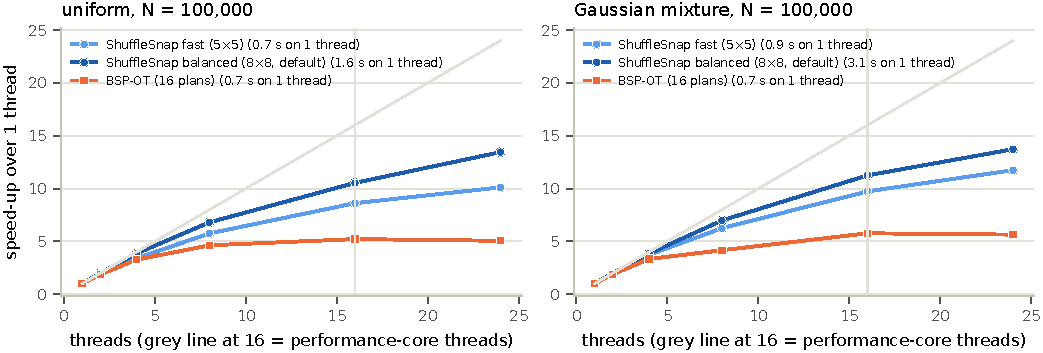
\includegraphics[width=\linewidth]{figures/fig_threads.pdf}
  \caption{Speed-up over one thread at $N=100{,}000$ (median of one run per setting,
  threads not pinned). The machine has 16 performance-core and 8 efficiency-core hardware
  threads; the light diagonal is linear speed-up. \ShuffleSnap's windows are independent
  within a phase, so it keeps scaling with the efficiency cores. BSP-OT stops improving
  at 8--16 threads, because its plans run in parallel but the merge that combines them is
  largely sequential.}
  \label{fig:threads}
\end{figure}

Figure~\ref{fig:threads} shows parallel scaling. \ShuffleSnap\ doubles its speed with each
doubling of threads up to 8 (7.7$\times$ at 8 threads). It reaches 12.5$\times$ at 16 and
14.8$\times$ at 24, with the same assignment at every thread count. BSP-OT reaches about
5--6$\times$ at 16 threads and gains nothing from the efficiency cores. We did not profile
where \ShuffleSnap\ loses efficiency beyond 8 threads. The efficiency cores are slower than
the performance cores, and each phase ends with a synchronization point.
